\chapter{一元函数}\label{chap:one_variable_functions}

\section{函数概念}\label{sec:function_concept}


\subsection{变量及其变动区域}\label{subsec:variables_and_ranges}
在 \emph{\ref{subsec:22}} 中, 我们已经介绍了变量的一般概念.
设数集 $\X=\{x\}$ 给出了变量 $x$ 在所考察问题中可能取得的全部数值,
并且其中每一个数值都允许取到,
这个数集就称为变量 $x$ 的\emph{变动区域}\index{biandongquyu@变动区域},
也就是变量的取值范围.
一般来说, 任意数集都可以作为某个变量的变动区域
\footnote{对数列而言, 仅给出所有可能的取值还不能确定这个数列,
因为各项的先后次序和重复情况同样是数列的组成部分
[参见 \emph{\ref{subsec:22}}].}.

我们已经讲过, 数可以表示为数轴上的点, 因此数集 $\X$ 也可以看成数轴上的一个点集.
在这种几何解释下, 变量所取的数值通常也称为点.

例如, 变量 $n$ 可以以自然数集 $\N$ 为变动区域.
数列
$
x_n=\dfrac{1+(-1)^n}{n}
$
取得的不同数值则构成数集
\footnote{若把数列看成定义在 $\N$ 上的函数,
则应当区分它的定义域 $\N$ 与它实际取得的值域.
本书以后讨论数列时, 不再使用“数列的变动区域”这一说法
[参见 \emph{\ref{subsec:function_definition}}].}
$
\left\{0,1,\dfrac12,\dfrac13,\ldots\right\}.
$
常量也可以看成变量的特殊情形, 它的变动区域只含一个数.

分析学中通常考察连续变动的变量.
时间、运动点经过的路程等物理量, 都是这类变量的典型例子.
对这类变量而言, 最常用的变动区域是\emph{有限区间}\index{youxianqujian@有限区间},
它由两个实数 $a,b$ 作为为区间的端点或边界 (通常假设 $a<b$).
按照是否包含端点, 有限区间分为以下几种形式:
\begin{align*}
&\text{\emph{闭区间}}\index{biqujian@闭区间}
&&[a,b]=\{x:a\leqslant x\leqslant b\},\\
&\text{\emph{半开区间}}\index{bankaqujian@半开区间}
&&(a,b]=\{x:a<x\leqslant b\},\\
&&&[a,b)=\{x:a\leqslant x<b\},\\
&\text{\emph{开区间}}\index{kaiqujian@开区间}
&&(a,b)=\{x:a<x<b\}.
\end{align*}
在每一种情形中, $b-a$ 都称为区间的长度.
很容易想象, 在数轴上, 有限区间表示为一条线段;
区间是否包含端点, 对应于线段是否包含相应的端点.

有时还需要考察\emph{无穷区间}\index{wuqiongqujian@无穷区间}.
它们用“广义的数” $-\infty,+\infty$ 作为一端或两端, 记法与有限区间相似.
例如, $(-\infty,+\infty)$ 表示全体实数,
$(a,+\infty)$ 表示满足 $x>a$ 的全体实数,
$(-\infty,b]$ 表示满足 $x\leqslant b$ 的全体实数.
在数轴上, 无穷区间表示为向两端无限延伸的直线, 或向一端无限延伸的射线.

\subsection{变量间的函数关系，例题}\label{subsec:functional_relations_examples}
数学分析主要研究的不是某一个变量的独立变化,
而是两个或多个变量同时变化时彼此之间的关系.
这里先考察两个变量的最简单情形.

在数学、物理学、工程学以及日常生活中,
我们经常遇到同时变动的两个量.
它们并不能各自任意取值:
相反地,
当其中一个变量 (\emph{自变量}\index{zibianliang@自变量}) 的值给定后,
另一个变量 (\emph{因变量}\index{yinbianliang@因变量}或\emph{函数}\index{hanshu@函数}) 的值也随之确定了.
下面先看几个例子.

\myrefparagraph{1)}\label{ex:circle_area_function}
圆的面积 $Q$ 是其半径 $R$ 的函数.
给定 $R$ 后, $Q$ 由公式
$$
Q=\pi R^2
$$
唯一确定.

\myrefparagraph{2)}\label{ex:free_fall_function}
忽略空气阻力时, 质点从静止开始自由落下.
从运动开始计时, 经过时间 $t$ 后的路程 $s$ 满足
$$
s=\frac{gt^2}{2},
$$
其中 $g=9.81\,\mathrm{m/s^2}$ 为重力加速度.
因此, 路程 $s$ 就成为经过的时间 $t$ 的函数.

\myrefparagraph{3)}\label{ex:boyle_mariotte_function}
一定质量的理想气体密闭在带活塞的气缸中.
温度保持不变时, 气体的体积 $V$ 与压力 $p$ 遵循 Boyle--Mariotte 定律: $pV=c=$ 常数.
于是给定体积 $V$ 后, 压力由
$$
p=\frac{c}{V}
$$
唯一确定, 因而 $p$ 是 $V$ 的函数.

\myrefparagraph{4)}\label{ex:barometric_function}
再考察大气压力 $p$ 与海拔高度 $h$ 的关系.
物理学给出气压公式
$$
p=p_0\e^{-kh},
$$
其中 $p_0$ 是海平面处的气压, $k$ 是常量.
若给定高度 $h$, 上式就把 $p$ 表示为 $h$ 的函数.

最后, 还应该有这个概念, 在两个相互关联的变量中, 选哪一个作为自变量并非总是固定的.
实际选择通常由研究目的和计算上的便利决定.
例如对于最后的例子, 一个飞行师若要根据气压计的读数 $p$ 来确定此时的飞行高度,
就应交换两个变量的角色, 将同一关系写成
$$
h=\frac{1}{k}\ln\frac{p_0}{p}.
$$
其它的例子也有类似的写法.
需要注意的是,
最开始的两个例子中, 我们交换两个变量后,
理论上对应于一个自变量, 有两个自变量 (一正一负) 随之确定,
这个时候, 我们还需要关注新的因变量 (长度 $R$ 与 时间 $t$) 的实际意义,
它们通常意义下只能选取正的情况.


\subsection{函数概念的定义}\label{subsec:function_definition}
现在我们抽去上述各个量的具体物理意义, 来给出函数概念的一般定义.

{\kaishu 设 $\X,\Y$ 是两个给定的数集,
如果按照某一确定的对应法则 $f$,
对每一个 $x\in\X$, 都有唯一确定的 $y\in\Y$ 与之对应,
那么称 $f$ 是从 $\X$ 到 $\Y$ 的函数, 记作
$$
f:\X\to\Y,
$$
并写成 $y=f(x)$}.
自变量 $x$ 也称为函数的\emph{变元}\index{bianyuan@变元},
$y=f(x)$ 称为函数在 $x$ 处的\emph{函数值}\index{hanshuzhi@函数值}.

在这个定义中存在两个要素:
第一, 指出变元 $x$ 的变动区域 $\X$ (它称为函数 的\emph{定义域}\index{dingyiyu@定义域});
第二, 确定 $x$ 与 $y$ 的数值之间的对应法则或规律
(函数 $y$ 的变动区域 $\Y$ 通常并不指出, 因为对应的规律本身就已经确定函数值的集合了
\footnote{在现代集合论的语言中,
我们将 $\Y$ 称为函数的\emph{陪域}\index{peiyu@陪域},
所有实际函数值构成的集合 $f(\X)=\{f(x):x\in\X\}$ 称为函数的\emph{值域}\index{zhiyu@值域},
后者是 $\Y$ 的子集, 但未必等于 $\Y$.
例如, $f$ 是恒等于零的一个函数, 那么它的值域由唯一的零构成, 但是其变动区域则可以是任意一个含有零的集合.
}).

按照定义, 每个 $x\in\X$ 只能对应一个函数值.
但是我们也可以建立更为普遍的观点上, 就是假设同一个 $x$ 允许对应多个 $y$,
在这种场合函数就称为\emph{多值函数}\index{duozhihanshu@多值函数},
用以区分前面所定义的\emph{单值函数}\index{danzhihanshu@单值函数}.
然而, 在分析学中, 如果我们的变量都取值于实数, 大多不讨论多值函数的情况,
以后说到函数, 如无特别说明, 我们始终理解成单值函数.

我们通常用不同的字母 $f,\varphi,F,\ldots$ 表示不同的对应法则
如果同时考察具有同一自变量的几个不同函数,
就应当用不同的字母区分它们:
$$
y=f(x),\qquad y=\varphi(x),\qquad y=F(x),\quad\ldots.
$$
有时我们就直接重复用着字母 $y$, 记成 $y=y(x)$.

某些情形下, 也会把自变量写成下标,
数列的记号 $x_n$ 就属于这种形式, 它是自变量 $n$ 的函数, 而 $n$ 则取值于自然数集 $\N$.
类似地 $N_\epsilon$ 的记法 [\emph{\ref{subsec:23}}] 表示序号 $N$ 依赖着 $\epsilon$, 等等.

若要指出函数 $f$ 对应于某个特定自变量值 $x_0$ 的函数值,
就写成 $f(x_0)$.
例如, 若
$$
f(x)=\frac{1}{1+x^2},\qquad
g(t)=\frac{10}{t},\qquad
h(u)=\sqrt{1-u^2},
$$
则 $f(1)$ 表示 $f(x)$ 在 $x=1$ 时的函数值, 即化简后的数 $\dfrac{1}{2}$,
类似地, $g(5)=2, h\brac{\dfrac35}=\dfrac45$ 等等.

函数对应法则的给出方式可以多种多样.
最简单也最常用的方式,
是用\emph{解析式}\index{jiexishi@解析式}或\emph{公式}\index{gongshi@公式}说明应对 $x$ 作哪些运算才能得到 $y$.
这种\emph{解析表示法}\index{jiexibiaoshifa@解析表示法}是数学分析中最重要的方法 (我们将在下一小节讨论),
我们在 \emph{\ref{subsec:functional_relations_examples}} 中讲述的四个例题都采用了这种解析表示.

然而, 解析式并不是表示函数的唯一方法, 在数学内也有很多函数是无法用公式来定义的.
例如, 常用的取整函数 $\floor{x}$
\footnote{参见 \emph{\ref{subsec:25}} 中例 \ref{ex:infinitesimal_basic_sequences} 的脚注.},
它就无法给出一个单一的算式.

还有许多只在自然数上取值的“算术函数,
例如阶乘 $n!=1\cdot2\cdots n$,
正因数个数函数 $\tau(n)$,
以及表示 $1,2,\ldots,n$ 中与 $n$ 互素的整数个数的 Euler 函数 $\varphi(n)$.

在自然科学和工程学中, 变量间的函数关系还常由实验或观测确定.
例如, 对任意选定的大气压力 $p$, 实验都可测得与之对应的水的沸点温度 $\theta$;
因此 $\theta$ 是 $p$ 的函数.
这种关系未必由一个公式表示, 也可以用实验数据表给出.
这种\emph{列表法}\index{liebiaofa@列表法}给定函数的实例在任何工程手册上都很容易找到.

最后, 函数关系还可以直接用\emph{图像}\index{tuxiang@图像}表示.
例如, 蒸汽机的指示器所画出的指示图,
表示汽缸内蒸汽压力 $p$ 与体积 $V$ 之间的关系;
气压自记器得到的气压图, 则表示大气压力在昼夜间的变化.
函数的表格表示和图形表示在分析中并非始终必须,
因而这里不再详细展开.

\subsection{函数的解析表示法}\label{subsec:analytic_representation}
函数的解析式或公式的表示法在数学分析中起着极其重要的作用.
下面先对这种表示法作几点说明.

\myrefparagraph{1\textdegree}\label{par:analytic_operations}
首先要说明, 解析式中允许进行哪些运算.
除初等代数和三角学中已经研究过的算术运算、乘幂、开方、取对数、求三角函数值及其反运算外,
还要加入我们在第一章中引入的一种新的运算 —— 极限运算.
随着分析学内容的展开, 还会逐步引入新的运算,
因此“解析式”或“公式”的完整含义也只能逐步揭示.

\myrefparagraph{2\textdegree}\label{par:natural_domain}
其次要注意解析式所表示的函数的定义域.
每一个含有自变量 $x$ 的解析式都有一个自然定义域,
即使这个解析式具有意义的一切实数 $x$ 所组成的集合
\footnote{对于任何实数 $x$ 都没有意义的解析式, 这里不加讨论.}.

例如, 表达式 $\dfrac{1}{1+x^2}$ 的自然定义域是全体实数 $\R$;
$\sqrt{1-x^2}$ 的自然定义域是闭区间 $[-1,1]$,
而 $\dfrac{1}{\sqrt{1-x^2}}$ 的自然定义域是开区间 $(-1,1)$.
有时自然定义域由几个彼此分离的区间组成:
$\sqrt{x^2-1}$ 的自然定义域是 $(-\infty,-1]$ 和 $[1,+\infty)$,
而 $\dfrac{1}{x^2-1}$ 的自然定义域则是 $(-\infty,-1)$, $(-1,1)$ 和 $(1,+\infty)$.

再考察无穷几何级数的和
$$
1+x+x^2+\cdots
=\lim_{n\to\infty}\brac{1+x+x^2+\cdots+x^{n-1}}
$$
若 $\abs{x}<1$, 则我们知道 [\emph{\ref{subsec:25}}, \ref{ex:geometric_series_sum}], 
它有极限 $\dfrac{1}{1-x}$, 
而当 $\abs{x}\geqslant1$ 时, 上式中的极限或者等于 $+\infty$, 或者根本不存在.
因此这个解析式的自然定义域是开区间 $(-1,1)$.

以后我们还会遇到更复杂、更一般的解析式,
并研究它们在自然定义域内所确定的函数的性质, 即研究解析工具本身.
不过, 在具体问题中还可能出现另一种情形:
自变量 $x$ 由于问题本身的性质而被限制在某个变动区域 $\X$ 内,
即使解析式在 $\X$ 以外仍有意义, 也不能越出这个区域来讨论原问题.
例如, 在自由落体问题 [\emph{\ref{subsec:functional_relations_examples}}, \ref{ex:free_fall_function}] 中,
质点从地面以上高 $h$ 处开始下落, 路程由公式
$$
s=\frac{gt^2}{2}
$$
给出. 这个解析式对于一切实数 $t$ 都有意义,
但原问题只允许考察
$$
0\leqslant t\leqslant T,\qquad T=\sqrt{\frac{2h}{g}}.
$$
负的时间没有实际意义; 当 $t>T$ 时, 质点已经落到地面.
在这里, 解析式只起辅助作用, 函数实际考察的定义域由具体问题限定.

\myrefparagraph{3\textdegree}\label{par:piecewise_analytic_representation}
最后, 函数未必在整个定义域内由同一个公式给出,
而是对于变元的某一部分数值用某一公式，对于另一部分数值用另一公式
例如, 在区间 $(-\infty,+\infty)$ 上定义函数
$$
f(x)=
\begin{cases}
1, & \abs{x}>1,\\
-1, & \abs{x}<1,\\
0, & x=\pm1.
\end{cases}
$$
这里对自变量的不同部分分别使用了不同的公式.

又如, \emph{Dirichlet 函数}\index{Dirichlethanshu@Dirichlet 函数}定义为
$$
D(x)=
\begin{cases}
1, & x\text{ 是有理数},\\
0, & x\text{ 是无理数}.
\end{cases}
$$
再如, \emph{符号函数}\index{fuhaohanshu@符号函数}也称为 Kronecker 函数, 记作 $\sgn x$:
$$
\sgn x=
\begin{cases}
1, & x>0,\\
-1, & x<0,\\
0, & x=0.
\end{cases}
$$

不过, 由几个公式分段定义的函数与由单一公式定义的函数之间并没有原则上的差别.
通常, 借助较为复杂的表达式, 可以把分段定义改写成一个公式.
例如, 利用极限运算, 上面引入的 $f(x)$ 可以写成
$$
f(x)=\lim_{n\to\infty}\frac{x^{2n}-1}{x^{2n}+1}.
$$
很容易检验, 当 $\abs{x}>1$ 时, $x^{2n}\to+\infty$, 因而
$$
\lim_{n\to\infty}\frac{x^{2n}-1}{x^{2n}+1}
=\lim_{n\to\infty}\frac{1-\dfrac{1}{x^{2n}}}{1+\dfrac{1}{x^{2n}}}=1.
$$
当 $\abs{x}<1$ 时, $x^{2n}\to0$, 所以
$$
\lim_{n\to\infty}\frac{x^{2n}-1}{x^{2n}+1}=-1.
$$
最后, 当 $x=\pm1$ 时, 对每个 $n$ 都有
$$
\frac{x^{2n}-1}{x^{2n}+1}=0,
$$
取极限后仍得 $0$. 这正好与原来的分段定义完全一致.

\subsection{函数的图像}\label{subsec:function_graph}
虽然在数学分析中并不用图像来给出函数,
但经常要借助图像说明函数的性质.
图像直观而清楚, 是研究函数性质时不可缺少的辅助工具.

\begin{wrapfigure}[7]{l}{0.34\textwidth}
    \vspace{-0.3cm}
    \centering
    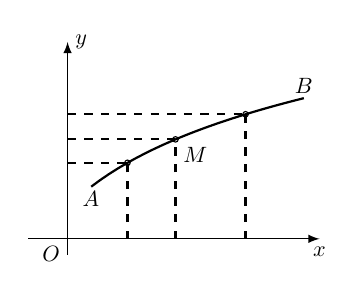
\begin{tikzpicture}
        \draw[-latex] (-0.5, 0) -- (3.2, 0) node[below,scale=0.8] {$x$};
        \draw[-latex] (0, -0.2) -- (0, 2.5) node[right,scale=0.8] {$y$};
        \node[below left,scale=0.8] (O) at (0, 0) {$O$};

        \node[below left,scale=0.8] (A) at (0.5, 0.7055) {$A$};
        \node[above,scale=0.8] (B) at (3, 1.75) {$B$};
        \node[below right,scale=0.8] (M) at (1.37, 1.2629) {$M$};

        \draw[domain=0.3:3, thick] plot (\x, {ln(\x+1)+0.4});

        \draw[dashed,thick] (0.76, 0) -- (0.76, 0.9653);
        \draw[dashed,thick] (1.37, 0) -- (1.37, 1.2629);
        \draw[dashed,thick] (2.26, 0) -- (2.26, 1.5817);
        \draw[dashed,thick] (0, 0.9653) -- (0.76, 0.9653);
        \draw[dashed,thick] (0, 1.2629) -- (1.37, 1.2629);
        \draw[dashed,thick] (0, 1.5817) -- (2.26, 1.5817);

        \draw (0.76, 0.9653) circle (1pt);
        \draw (1.37, 1.2629) circle (1pt);
        \draw (2.26, 1.5817) circle (1pt);
    \end{tikzpicture}
 \end{wrapfigure}
设函数 $y=f(x)$ 定义在某个区间 $\X$ 内.
在平面上取两条互相垂直的坐标轴, 对每一对满足 $x\in\X$、$y=f(x)$ 的数值,
作横坐标为 $x$、纵坐标为 $y$ 的点 $M(x,y)$.
当 $x$ 在 $\X$ 内变动时, 所有这些点组成的集合就是函数 $y=f(x)$ 的\emph{图像}.
在图示的情形中, 这些点画出一条曲线 $AB$;
这条曲线是函数的几何表示, 而方程 $y=f(x)$ 就称为曲线 $AB$ 的方程.

例如, 函数
$$
\begin{aligned}
y=\pm\sqrt{1-x^2}\quad (\abs{x}\leqslant1),\qquad
y=\pm\sqrt{x^2-1}\quad (\abs{x}\geqslant1)
\end{aligned}
$$
的图像分别是下方圆和等轴双曲线:

\begin{figure}[htbp]
    \vspace{-0.7cm}
    \centering
    \begin{minipage}[t]{0.44\textwidth}
        \centering
        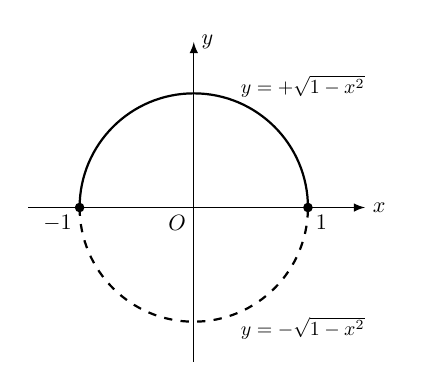
\begin{tikzpicture}[scale=1.45]
            \draw[-latex] (-1.45,0) -- (1.5,0) node[right,scale=0.8] {$x$};
            \draw[-latex] (0,-1.35) -- (0,1.45) node[right,scale=0.8] {$y$};
            \node[below left,scale=0.8] at (0,0) {$O$};
            \draw[thick] (1,0) arc[start angle=0,end angle=180,radius=1];
            \draw[dashed,thick] (-1,0) arc[start angle=180,end angle=360,radius=1];
            \fill (-1,0) circle (1.2pt);
            \fill (1,0) circle (1.2pt);
            \node[above right,scale=0.72] at (0.35,0.9) {$y=+\sqrt{1-x^2}$};
            \node[below right,scale=0.72] at (0.35,-0.9) {$y=-\sqrt{1-x^2}$};
            \node[below left,scale=0.8] at (-1,0) {$-1$};
            \node[below right,scale=0.8] at (1,0) {$1$};
        \end{tikzpicture}
    \end{minipage}
    \hfill
    \begin{minipage}[t]{0.48\textwidth}
        \centering
        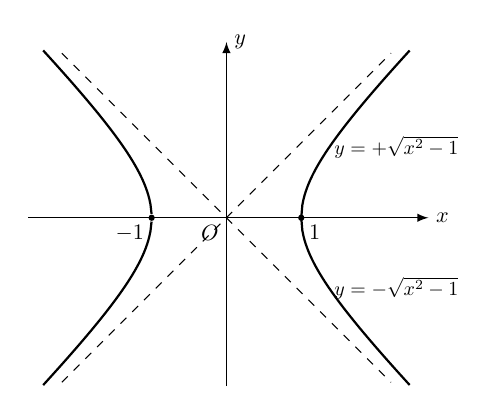
\begin{tikzpicture}[scale=0.95]
            \draw[-latex] (-2.65,0) -- (2.7,0) node[right,scale=0.8] {$x$};
            \draw[-latex] (0,-2.25) -- (0,2.35) node[right,scale=0.8] {$y$};
            \node[below left,scale=0.8] at (0,0) {$O$};
            \draw[dashed] (-2.2,-2.2) -- (2.2,2.2);
            \draw[dashed] (-2.2,2.2) -- (2.2,-2.2);
            \draw[domain=1:2.45,samples=100,thick] plot (\x,{sqrt(\x*\x-1)});
            \draw[domain=1:2.45,samples=100,thick] plot (\x,{-sqrt(\x*\x-1)});
            \draw[domain=-2.45:-1,samples=100,thick] plot (\x,{sqrt(\x*\x-1)});
            \draw[domain=-2.45:-1,samples=100,thick] plot (\x,{-sqrt(\x*\x-1)});
            \fill (-1,0) circle (1.2pt);
            \fill (1,0) circle (1.2pt);
            \node[above right,scale=0.72] at (1.35,0.7) {$y=+\sqrt{x^2-1}$};
            \node[below right,scale=0.72] at (1.35,-0.7) {$y=-\sqrt{x^2-1}$};
            \node[below left,scale=0.8] at (-1,0) {$-1$};
            \node[below right,scale=0.8] at (1,0) {$1$};
        \end{tikzpicture}
    \end{minipage}
\end{figure}

\begin{wrapfigure}[10]{r}{0.45\textwidth}
    \vspace{-0.5cm}
    \centering
    \begin{tikzpicture}[scale=0.85]
        \draw[-latex] (-2.65,0) -- (3.55,0) node[right,scale=0.8] {$x$};
        \draw[-latex] (0,-2.65) -- (0,2.85) node[right,scale=0.8] {$y$};
        \node[below left,scale=0.8] at (0,0) {$O$};
        \foreach \x in {-2,-1,1,2,3}{
            \draw (\x,0.08) -- (\x,-0.08) node[below] {$\x$};
        }
        \foreach \k in {-2,-1,0,1,2}{
            \draw[thick] (\k,\k) -- (\k+1,\k);
            \fill (\k,\k) circle (1.8pt);
            \draw[fill=white] (\k+1,\k) circle (1.8pt);
        }
        \node[left,scale=0.8] at (0,-2) {$-2$};
        \node[left,scale=0.8] at (0,-1) {$-1$};
        \node[left,scale=0.8] at (0,1) {$1$};
        \node[left,scale=0.8] at (0,2) {$2$};
        \node[above left,scale=0.8] at (-0.25,2.15) {$y=\floor{x}$};
    \end{tikzpicture}
\end{wrapfigure}
函数图像通常是逐点画出的.
在区间 $\X$ 内取一系列彼此接近的自变量值,
依公式 $y=f(x)$ 算出相应的函数值:
$$
\begin{array}{c|ccccc}
x= & x_1 & x_2 & x_3 & \cdots & x_n\\ \hline
y= & y_1 & y_2 & y_3 & \cdots & y_n
\end{array}
$$
再把点
$$
(x_1,y_1),\ (x_2,y_2),\ \ldots,\ (x_n,y_n)
$$
画在图上, 用光滑的线段连接作出曲线.
这样得到的曲线虽然只是所求图像的近似,
但是曲线画得越光滑, 所取的点越稠密, 它就越准确地表示函数的图像.

必须注意, 虽然常用几何图形来表示函数,
函数的图像却不一定是通常直观意义下的曲线.
例如, 取整函数 $y=\floor{x}$ 在每个区间 $[m,m+1)$ ($m$ 取一切整数) 内都保持常值 $m$,
因而它的图像由一系列左端点属于图像、右端点不属于图像的水平线段组成.
至于 Dirichlet 函数 $D(x)$,
它的图像由直线 $y=1$ 上横坐标为有理数的点,
以及 $x$ 轴上横坐标为无理数的点组成, 这种图像却无法实际画出.

\subsection{几类重要的函数}
